\ylDisplay{Golfilöök} % Ülesande nimi
{Tundamtu autor} % Autor
{lõppvoor} % Voor
{2012} % Aasta
{P 2} % Ülesande nr.
{1} % Raskustase
{
% Teema: Mehaanika

\ifStatement
Sarivõttega pildistati golfimängijat nii, et iga kahe pildi vahel oli ajavahemik $\tau = 16$ ms. Hinnake golfipalli algkiirust joonise abil. Pall liigub risti vaatesuunaga. Allpool on pilt.
\begin{center}
	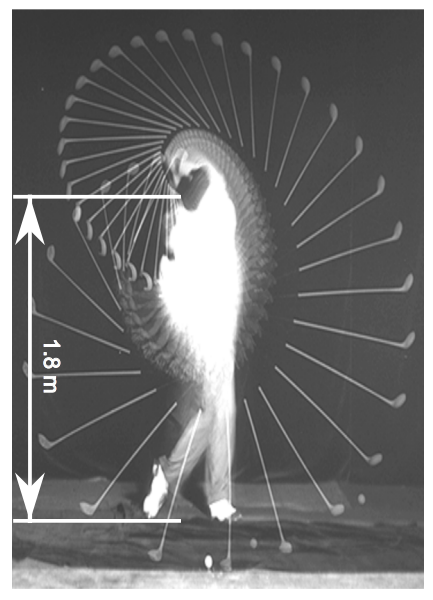
\includegraphics[width=0.5\linewidth]{2012-v3p-02-yl.PNG}
\end{center}
\fi

\ifHint
Tuleb võtta arvesse, et heledaim valge täpp meile infot ei anna, sest see näitab vaid golfipalli algasendit enne seda, kui kepp teda lõi. Kahele järjestikkusele pildile on jäädvustunud heledast pallist paremale jäävad kaks tuhmimat valget palli kujutist. Nende ajaline vahe on $\tau$ ning me saame mõõta pallide vahekauguse joonlauaga.
\fi

\ifSolution
Lendu läinud golfipall on pildile jäädvustunud kolmes punktis. Paneme tähele, et heledaim valge täpp meile aga infot ei anna, sest see näitab vaid golfipalli algasendit enne seda, kui kepp teda lõi! Kahele järjestikkusele pildile on jäädvustunud heledast pallist paremale jäävad kaks tuhmimat valget palli kujutist. Nende ajaline vahe on $\tau$ . Mõõdame pallide vahekauguse $L_1$ joonlauaga. Samuti mõõdame golfimängija pikkust märkivat skaalat või golfimängija pikkust $L_2$. Teades, et skaalajoone pikkusele vastab $h = 1,8$ m saame, et golfipalli nihke pikkus kahe pildi vahel on
\begin{center}
$s = \frac{hL_1}{L_2}$
\end{center}
Selleks nihkeks kulunud aeg oli $\tau$ . Kuna golfipalli kiirus on suur, siis raskuskiirendusega me ei arvesta, loeme, et tegu on kulgliikumisega. Kiiruseks saame
\begin{center}
$v = \frac{s}{\tau} = \frac{hL_1}{\tau L_2} \approx 150$ km/h.
\end{center}
\fi
}
